\setAuthor{Stanislav Zavjalov}
\setRound{lõppvoor}
\setYear{2011}
\setNumber{G 2}
\setDifficulty{2}
\setTopic{Dünaamika}

\prob{Varras}
Mööda liigendi abil seina külge kinnitatud väga pikka ja tühiselt
kerget varrast saab libiseda väike rõngas massiga $m$. Esialgu asub rõngas liigendist kaugusel $l$ ja varras on horisontaalne. Ajahetkel $t = \num{0}$ hakkab süsteem
vabalt liikuma. Leidke varda ja horisontaali vahelise nurga $\alpha$ ajaline sõltuvus.
Kõik liikumised lugeda hõõrdevabaks. 

\hint
Ülesanne näeb keerulisem välja, kui see tegelikult on. Olukorda lihtsustab oluliselt asjaolu, et varras on tühiselt kerge ja libisemised hõõrdevabad.

\solu
\begin{center}
	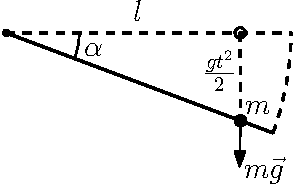
\includegraphics[width = 0.5\linewidth]{2011-v3g-02-varras_lah.pdf}
\end{center}

Kuna varras on kaalutu, peab sellele mõjuv summaarne jõud olema \num{0}. Vastasel korral mõjuks sellele Newtoni III seaduse kohaselt lõpmatu jõud, mis pole füüsikaline. Sellest saab järeldada, et massile mõjuv normaaljõud on null ning hõõrdeta libisemise tõttu on ka vardaga paralleelne jõukomponent null. Seega ei mõju massile varda poolt ükski jõud ning mass on vabalanguses. 

Aja $t$ jooksul jõuab mass langeda vahemaa $\frac{gt^2}{2}$ ning varda ja horisontaali vaheline nurk avaldub kui (vt joonist) $\tan\alpha = \frac{gt^2}{2l}$.\probend